
\documentclass[slidestop, compress, mathserif]{beamer}

\usepackage[style=authoryear-comp, sorting=nyt, maxcitenames=2, backend=biber]{biblatex}
\renewbibmacro{in:}{}
\renewcommand\bibfont{\small}
%% \addbibresource{ref.bib}

\usepackage{amsmath, amssymb, mathrsfs}
\usepackage{color, graphicx}

\usepackage{setspace, listings}
\usepackage{sidecap}

\usetheme{Madrid}
\usecolortheme{default}
\linespread{1.2}



\sidecaptionvpos{figure}{c}
\usepackage[textfont=small]{caption}
\setbeamertemplate{caption}[numbered]
\captionsetup{font=scriptsize, labelfont=scriptsize, labelformat=simple}

\setbeamertemplate{footline}
{
  \leavevmode%
  \hbox{%
  \begin{beamercolorbox}[wd=1.0\paperwidth,ht=2.25ex,dp=1ex]{author in head/foot}\usebeamerfont{author in head/foot}
    \hspace*{3ex}
    \inserttitle
    \hfill
    % \insertshortauthor
    % \insertfirstauthor
    Gun Woo Park 
    \hspace{1em}\insertshortdate
    \hspace{1em}\insertframenumber/\inserttotalframenumber
    \hspace*{3ex}
  \end{beamercolorbox}%
}%
  \vskip0pt%
}

\title{Dissociation Transition Probability}
%% \institute{DICMaPI, University of Naples Federico II}
%% \author{Gun Woo Park, Giovanni Ianniruberto, and Giuseppe Marrucci}
%% \date{13 APR 2016}
\author{Gun Woo Park}

% it's for headline
\setbeamertemplate{headline}{%
  % \leavemode%
  \hbox{%
    % \begin{beamercolorbox}[wd=\paperwidth,ht=2.5ex,dp=1.125ex]{palette quaternary}%
    \begin{beamercolorbox}[wd=\paperwidth,ht=2.5ex,dp=1.125ex]{section in head/foot}%
      \insertsectionnavigationhorizontal{\paperwidth}{}{\hskip0pt plus1filll}
    \end{beamercolorbox}%
    }
}

\begin{document}

\begin{frame}[plain]
  \maketitle
\end{frame}

\section{Original}
\begin{frame}
  \frametitle{Baisic Approaches}
  Let $N_{tot}$ be number of total chains on the system and $N^\dagger$ be number of activated (transition) chain ends. Originally, the dissociation transition probability is based on the expected value:
  \begin{equation}
    N^\dagger = N_{tot} \bar{\beta}\Delta t\label{eq:origin_probability},
  \end{equation}
  where $\bar{\beta}$ is the average detachment frequency of the system and $\Delta t$ is given time step for topological update.
  From here, we can define dissociation transition probability as
  \begin{equation}
    \frac{N^\dagger}{N_{tot}} = \bar{\beta}\Delta t \equiv P^{dissoc}.
  \end{equation}

\end{frame}

\begin{frame}
  For stochastic simulation, we are focused on the subjected chain end where the bridge information is given. Therefore, we can use following transition probability:
  \begin{equation}
    P^{dissoc}(r, \Delta t) = \min\{1, \beta(r)\Delta t\},
  \end{equation}
  where the truncate to unity is similar to the Metropolis-Hasting algorithm.

  Equation \eqref{eq:origin_probability} is based on 0-th order transition probability of following transition:
  \begin{equation}
    N_{passive} \xrightarrow{\beta} N^\dagger,
  \end{equation}
  where passive means both chain ends are attached and $\dagger$ means one of the chain end is in transit state. 
  If the transition is 0-th order, we have
  \begin{equation}
    \frac{d N^\dagger(t)}{dt} = \beta \Rightarrow N^\dagger(t) = N_{tot}\beta t\quad\textrm{for }t<\tau_0. \label{eq:0th_order}
  \end{equation}
\end{frame}

\section{First-Order}
\begin{frame}
  \frametitle{First-Order Approaches}
  It is of importance that the number of \textit{active} chain end depends on the number of suggestions (number of passive chain ends), which means it should be (at least) first-order rather than 0-th order, Eq. \eqref{eq:0th_order}. Therefore, we have
  \begin{equation}
    \frac{d N_{passive}(t)}{dt} = -\beta N_{passive} \Rightarrow N_{passive}(t) = N_{tot}\exp\left(-\beta t\right).
  \end{equation}
  Since $N^\dagger = N_{tot} - N_{passive}$, we have
  \begin{equation}
    N^\dagger(t) = N_{tot}\left(1 - \exp\left(-\beta t\right)\right) = N_{tot}\left(1 - \exp\left(-\frac{t}{\tau}\right)\right),
  \end{equation}
  which is the similar with Cifre et al. (2003).
\end{frame}

\begin{frame}
  It is of importance that the $\tau(r) = \beta(r)^{-1}$ is dissociation characteristic time for dissociation transition of subjected chain end. In addition, the 1st order scheme satisfies the conditional probabliity example. Let assumed that we have sufficient number chain end with the exactly the same chain end-to-end distance. Expected number of active chain end, of course, have dependence of time, which should follow conditional probability:
  \begin{equation}
    P^{dissoc}(r, t) = (P^{dissoc}(r, t/N))^{N}.
  \end{equation}
  It means when we allows N times of topological update up to time t, with fixed r, the dissociation transition probability should be the same with 1 time of topological update up to time t. The 0th order, however, fails to this scheme because
  \begin{equation}
    P^{dissoc}(r, t) = \beta(r)t \neq \beta(r)^{N}(t/N)^{N}.
  \end{equation}
  In the case of 1st order scheme, this conditional balance well matched since
  \begin{equation}
    P^{dissoc}(r, t) = 1. - \exp(\beta(r) t) = 1. - 
  \end{equation}
\end{frame}

\section{Compare}
\begin{frame}
  \frametitle{Expected Probability for 0th and 1st Order Schemes}
  \begin{figure}
    \centering
    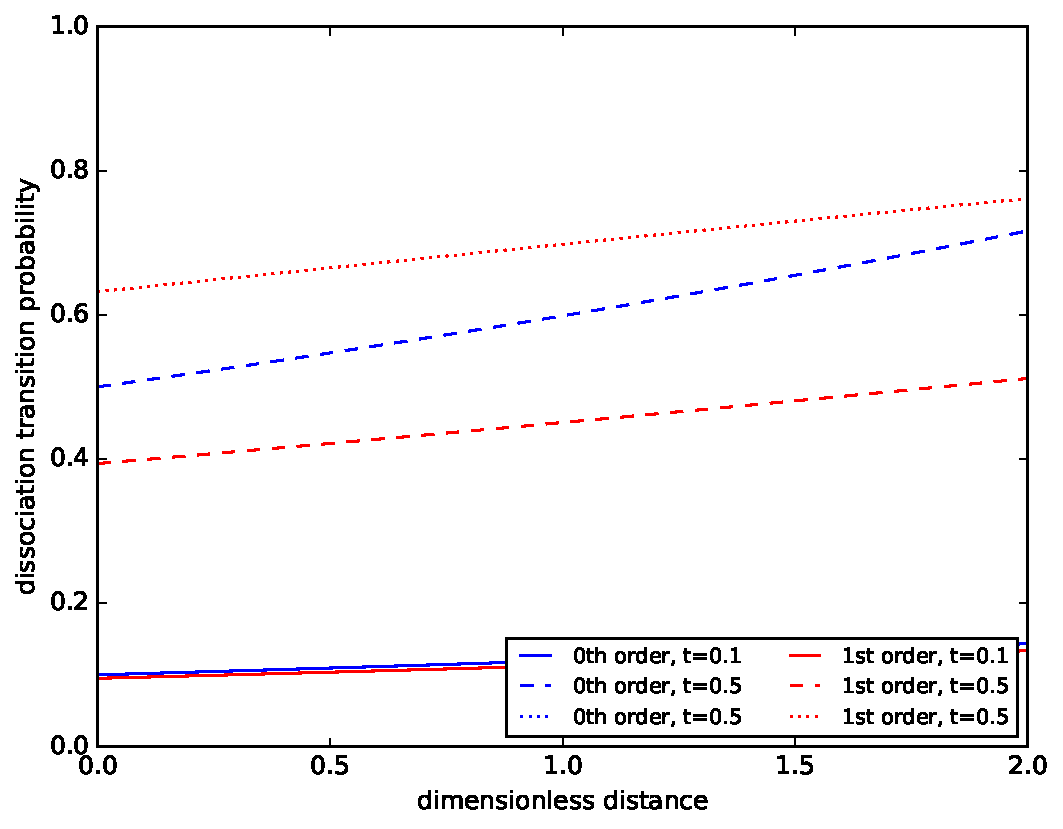
\includegraphics[width=0.45\textwidth]{../compare_dissociation_transition_probability_order.pdf}
    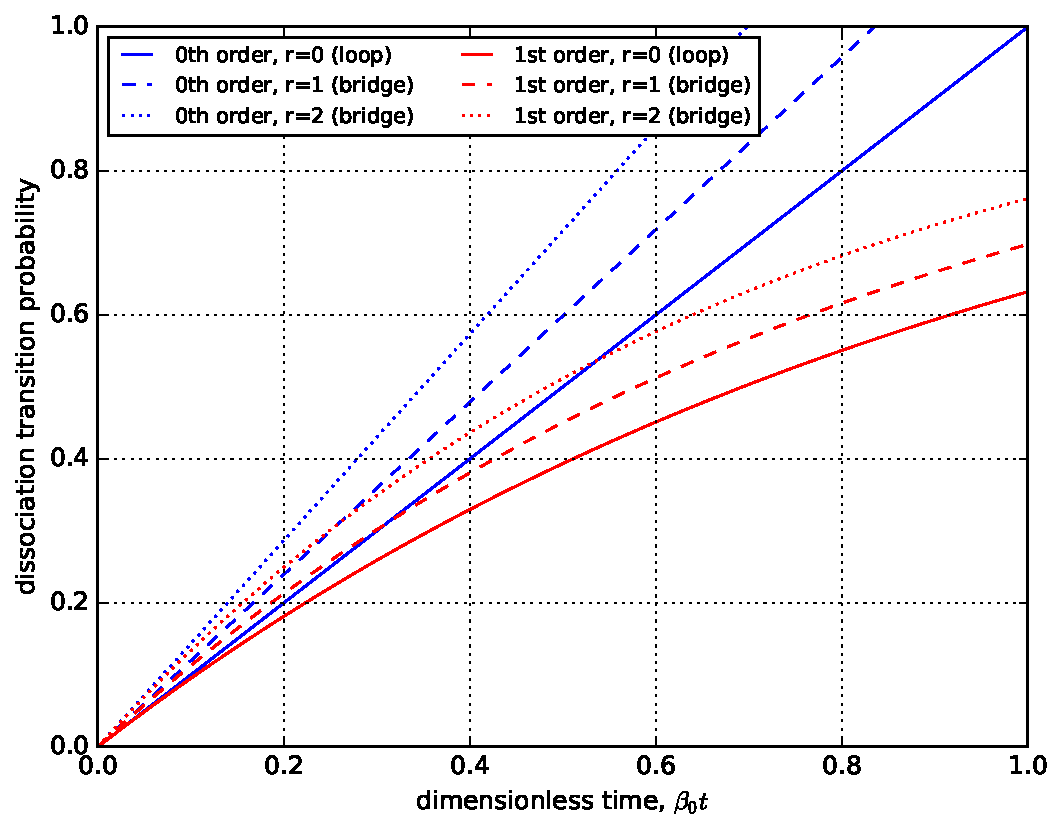
\includegraphics[width=0.45\textwidth]{../compare_dissociation_transition_probability_order_tdist.pdf}
    \caption{Comparison between the expected lines for the 0th order (blue) and 1st order (red) transition scheme.}
  \end{figure}
\end{frame}

\end{document}
%% \section{Overview}

%% \begin{frame}
%%   \frametitle{Introduction HEUR solution}
%%   \begin{figure}
%%     \centering
%%     \includegraphics[width=0.5\textwidth]{figures/structure_HEUR.png}
%%     \includegraphics[width=0.45\textwidth]{figures/dynamic_moduli_Suzuki_2012.png}
%%     \caption{Schematic diagram for HEUR solution (left) and dynamic moduli for HEUR solution in flower-like micelle regime (right, \textcite{Suzuki:2012gfa}).}
%%   \end{figure}
%% \end{frame}
%% \begin{frame}
%%   \frametitle{Linear Viscoelasticity and Concentration Dependence}
%%   \begin{figure}
%%     \centering
%%     \includegraphics[width=0.4\textwidth]{figures/dynamic_moduli_Uneyama_2012.png}    
%%     \includegraphics[width=0.3\textwidth]{figures/scaling_law_Uneyama_2012_a.png}
%%     \includegraphics[width=0.3\textwidth]{figures/scaling_law_Uneyama_2012_b.png}
%%     \caption{Linear viscoleasticity for HEUR solution.  \parencite{Suzuki:2012gfa}, the scaling law for dominant relaxation time (center) and plateau modulus (right) with respect to concentration \parencite{Uneyama:2012ge}.}
%%   \end{figure}
%% \end{frame}

%% \begin{frame}
%% \frametitle{Frictional and Topological Time Scales}
%% \begin{figure}
%%   \centering
%%   \includegraphics[width=0.49\textwidth]{figures/RTD_from_Uneyama.pdf}
%%   \includegraphics[width=0.49\textwidth]{figures/Gt_from_Uneyama.pdf}
%%   \caption{Calculated relaxation time spectrum (left) using dynamic moduli reported by \textcites{Suzuki:2012gfa, Uneyama:2012ge} based on fixed-point iteration method \parencite{SooCho:2013goa} and generated relaxation modulus (right) from its relaxation time spectrum.}
%% \end{figure}
%% \end{frame}

%% \begin{frame}
%%   \frametitle{Nonlinear Response for HEUR Solution}
%%   \begin{figure}
%%     \centering
%%     \includegraphics[width=0.49\textwidth]{figures/nonlinear_Suzuki_2012.png}
%%     \includegraphics[width=0.49\textwidth]{figures/nonlinear_viscosity_Suzuki_2012.png}
%%     \caption{Shear thickening for steady-state viscosity, $\eta(\dot{\gamma})$, while linearity for the first normal stress different coefficient before shear-thinning, $\Psi_1(\dot{\gamma})$, (left) and strain hardening for viscosity growth function, $\eta^+(t;\dot{\gamma})$, (right) \parencite{Suzuki:2012gfa}.}
%%   \end{figure}
%% \end{frame}

%% \begin{frame}
%%   \frametitle{Micelle Interaction Model}
%%   \begin{figure}
%%     \centering
%%     \includegraphics[width=0.49\textwidth]{figures/shear_thickening_Ianniruberto_2015.png}
%%     \includegraphics[width=0.49\textwidth]{figures/viscosity_growth_Ianniruberto_2015.png}
%%     \caption{Shear thickening for both of steady-state viscosity and the first normal stress different coefficient (left) and strain hardening for viscosity growth function (right) \parencite{Ianniruberto:2015dv}}
%%   \end{figure}
%% \end{frame}



%% \section{Methodology}
%% \begin{frame}
%%   \frametitle{Time Evolution for Frictional and Topological Dynamics}
%%   \begin{minipage}{0.45\textwidth}
%%     \begin{figure}
%%       \centering
%%       \includegraphics[width=\textwidth]<1>{figures/time_evolution_1.png}
%%       \includegraphics[width=\textwidth]<2>{figures/time_evolution_2.png}
%%       \includegraphics[width=\textwidth]<3>{figures/time_evolution_3.png}
%%       \includegraphics[width=\textwidth]<4>{figures/time_evolution_4.png}
%%       \caption{Schematic diagram for time evolution}
%%     \end{figure}
%%   \end{minipage}
%%   \begin{minipage}{0.5\textwidth}
%%     \only<1,2>{
%%       \begin{block}{Langevin Equation}
%%         \vspace{-0.1in}
%%         %% \begin{align*}
%%         %%   \zeta \frac{\partial \mathbf{r}_k}{\partial t} &= \mathbf{F}^{(B)}(\mathbf{r}_k) \nonumber\\
%%         %%   &+ \sum_{i=1}^{N_p}\mathbf{F}^{(rep)}(\mathbf{r}_i, \mathbf{r}_k) \nonumber\\
%%         %%   &+ \sum_{i\in \mathscr{C}_k} \mathbf{F}^{(el)}(\mathbf{r}_i, \mathbf{r}_k)
%%         %% \end{align*}
%%         \begin{equation*}
%%           \zeta \frac{\partial \mathbf{r}_k}{\partial t} = \sum_{i=1}^{N_p}\mathbf{F}^{(rep)}_{ik} + \sum_{i\in \mathscr{C}_k} \mathbf{F}^{(el)}_{ik} + \mathbf{F}^{(B)}_{k},
%%         \end{equation*}
%%         where the connectivity information given by topology, $\{\mathscr{C}_k\}$, is fixed.
%%       \end{block}
%%       Time step for Langevin equation: $dt=10^{-4}\tau_B = 10^{-4}\frac{\tau_B}{\tau_0}\tau_0\approx 10^{-6}\tau_0$.

%%     }
%%     \only<3>{
%%       \begin{block}{Dissociation Probability}
%%         \vspace{-0.1in}
%%         \begin{align*}
%%           P_{ij}^{dissoc} &= \frac{N^\dagger}{N_{tot}}\frac{\beta_{ij}}{\bar{\beta}} = \beta_{ij}\delta t,
%%         \end{align*}
%%         where $\delta t$ is time interval to update topology, and
%%         \vspace{-0.1in}
%%         \begin{align*}
%%           \beta_{ij} &\equiv \beta_0\exp\left(\frac{F^{(el)}_{ij}l_c}{k_BT}\right) \\
%%           N^\dagger &= N_{tot}\bar{\beta}\delta t
%%         \end{align*}
%%       \end{block}
%%     }
%%     \only<4>{
%%       \begin{block}{Association Map}
%%         Detached chain end immediately attaches to a bead using Boltzmann distribution:
%%         \begin{equation*}
%%           P_{ij} = \frac{1}{Z_j}\exp\left(-\frac{U_{ij}}{k_BT}\right)
%%         \end{equation*}
%%       \end{block}
%%       }
%%     %% \begin{block}<4>{Association probability}
%%     %% \end{block}
    
%%   \end{minipage}
%% \end{frame}

%% %% \section{Methodology}
%% %% \begin{frame}
%% %%   \frametitle{Time Evolution for Frictional Dynamics}
%% %%   \begin{minipage}{0.48\textwidth}
%% %%     \begin{figure}
%% %%       \centering
%% %%       \includegraphics[width=\textwidth]{figures/time_evolution_2.png}
%% %%       \caption{Schematic diagram for the given topology}
%% %%     \end{figure}
%% %%   \end{minipage}\hspace{0.2in}
%% %%   \begin{minipage}{0.45\textwidth}
%% %%     \begin{block}{Langevin Equation}
%% %%     \begin{align*}
%% %%       \zeta \frac{\partial \mathbf{r}_k}{\partial t} &= \sum_{i\in \mathscr{C}_k} \mathbf{F}^{(el)}(\mathbf{r}_i, \mathbf{r}_k) \nonumber\\
%% %%       &+ \sum_{i=1}^{N_p}\mathbf{F}^{(rep)}(\mathbf{r}_i, \mathbf{r}_k) \nonumber\\
%% %%       &+ \mathbf{F}^{(B)}(\mathbf{r}_k)
%% %%     \end{align*}
%% %%     \end{block}
%% %%   \end{minipage}
%% %% \end{frame}

%% %% \section{Methodology}
%% %% \begin{frame}
%% %%   \frametitle{Time Evolution for Topology}
%% %%   \begin{minipage}{0.48\textwidth}
%% %%     \begin{figure}
%% %%       \centering
%% %%       \includegraphics[width=\textwidth]{figures/time_evolution_3.png}
%% %%       \caption{Schematic diagram for the given topology}
%% %%     \end{figure}
%% %%   \end{minipage}
%% %%   \begin{minipage}{0.5\textwidth}
%% %%     %% \begin{align}
%% %%     %%   \zeta \frac{\partial \mathbf{r}_k}{\partial t} &= \sum_{i\in \mathscr{C}_k} \mathbf{F}^{(el)}(\mathbf{r}_i, \mathbf{r}_k) \nonumber\\
%% %%     %%   &+ \sum_{i=1}^{N_p}\mathbf{F}^{(rep)}(\mathbf{r}_i, \mathbf{r}_k) \nonumber\\
%% %%     %%   &+ \mathbf{F}^{(B)}(\mathbf{r}_k)
%% %%     %% \end{align}
%% %%     \begin{block}{Dissociation probability}
%% %%     \begin{align}
%% %%       P_{ij} &= \frac{N^\dagger}{N_tot}\frac{\beta_{ij}}{\bar{\beta}} = \beta_{ij}\delta t \\
%% %%       \beta_{ij} &\equiv \beta_0\exp\left(\frac{F^{(el)}(\mathbf{r}_{ij})l_c}{k_BT}\right) \\
%% %%       N^\dagger &= N_{tot}\bar{\beta}\delta t
%% %%     \end{align}
%% %%     \end{block}
%% %%   \end{minipage}
%% %% \end{frame}

%% %% \section{Methodology}
%% %% \begin{frame}
%% %%   \frametitle{Time Evolution for Frictional Dynamics}
%% %%   \begin{minipage}{0.48\textwidth}
%% %%     \begin{figure}
%% %%       \centering
%% %%       \includegraphics[width=\textwidth]{figures/time_evolution_4.png}
%% %%       \caption{Schematic diagram for the given topology}
%% %%     \end{figure}
%% %%   \end{minipage}
%% %%   \begin{minipage}{0.5\textwidth}
%% %%     \begin{align}
%% %%       \zeta \frac{\partial \mathbf{r}_k}{\partial t} &= \sum_{i\in \mathscr{C}_k} \mathbf{F}^{(el)}(\mathbf{r}_i, \mathbf{r}_k) \nonumber\\
%% %%       &+ \sum_{i=1}^{N_p}\mathbf{F}^{(rep)}(\mathbf{r}_i, \mathbf{r}_k) \nonumber\\
%% %%       &+ \mathbf{F}^{(B)}(\mathbf{r}_k)
%% %%     \end{align}
%% %%   \end{minipage}
%% %% \end{frame}

%% %% \begin{frame}

%% %% \frametitle{Time Evolution for Frictional and Topological Dynamics}
%% %% \begin{block}{Fast Process: Network-Node Dynamics (Langevin Equation)}
%% %%   \begin{equation}
%% %%     \frac{\partial \mathbf{r}_k}{\partial t} = \frac{1}{\zeta} \left(\sum_{i\in \mathscr{C}_k} \mathbf{F}^{(el)}(\mathbf{r}_i, \mathbf{r}_k) + \sum_{i=1}^{N_p}\mathbf{F}^{(rep)}(\mathbf{r}_i, \mathbf{r}_k) + \mathbf{F}^{(B)}(\mathbf{r}_k)\right),
%% %%   \end{equation}
%% %%   where (el), (rep), and (B) represent elastic, repulsive, and Brownian contributions, respectively.
%% %% \end{block}

%% %% \end{frame}

%% %% \begin{frame}
%% %% % \begin{block}{Slow Process: Association/Dissociation Kinetics}
%% %% %   The dissociation transition probability is given by
%% %% %   \begin{equation}
%% %% %     P^{dissoc} = \beta \delta t = \beta_0 \exp\left(\frac{F^{(el)}l_c}{k_BT}\right),
%% %% %   \end{equation}
%% %% %   and the association following Boltzmann distribution.
%% %% % \end{block}
%% %% % \end{frame}
%% %% \begin{block}{Slow Process: Association/Dissociation Kinetics}
%% %%   For given position, we randomly select a chain end and check the dissociation transition probability
%% %%   \begin{equation}
%% %%     P^{dissoc} = \beta \delta t = \beta_0 \exp\left(\frac{F^{(el)}l_c}{k_BT}\right),
%% %%   \end{equation}
%% %%   where $\beta$ is the chain detachment frequency, accounting for a thermal non-activated process (with frequency $\beta_0$) amplified by the elastic contribution ($l_c$ being related to the length of the hydrophobic part). Once a chain end detaches, it immediately attaches based on Boltzmann distribution.

%% %% % If the chain detached, it immediately attached to a neighboring flower using index function based on Boltzmann distribution:
%% %% %   \begin{equation}
%% %% %     \mathscr{I}(p) = \left\{\begin{array}{cc} 1 & \textrm{if }p < F_j(1) \\
%% %% %                               2 & \textrm{if } F_j \leq p < F_j(2) \\
%% %% %                               \vdots & \vdots \\
%% %% %                               N_p & \textrm{if } F_j(Np-1) \leq p. \end{array}\right.
%% %% %   \end{equation}
%% %% \end{block}
%% %% \end{frame}

%% \section{Results}
%% \begin{frame}
%% \frametitle{Network Structures}
%% \begin{figure}
%%   \centering
%%   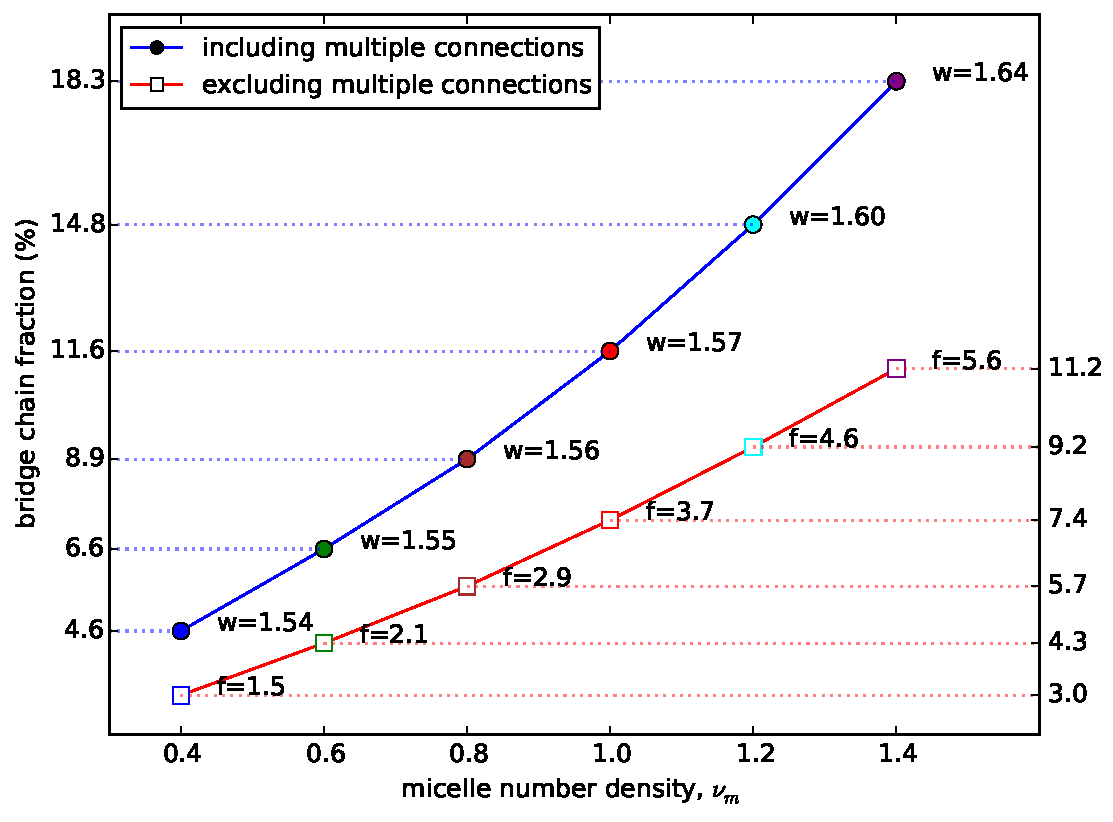
\includegraphics[height=0.6\textheight]{figures/bridge_chain_fraction_SUPOLEN_Leeds.pdf}
%%   \includegraphics[width=0.35\textwidth]{figures/exam_structure.png}
%%   \caption{Bridge chain fraction including and excluding multiple connections (left). Snap shot for $\nu_m=0.4$ is reported as example (right).}
%% \end{figure}
%% \end{frame}

%% \begin{frame}
%%   \frametitle{Pair-Correlation Function}
%%   \begin{figure}
%%     \centering
%%     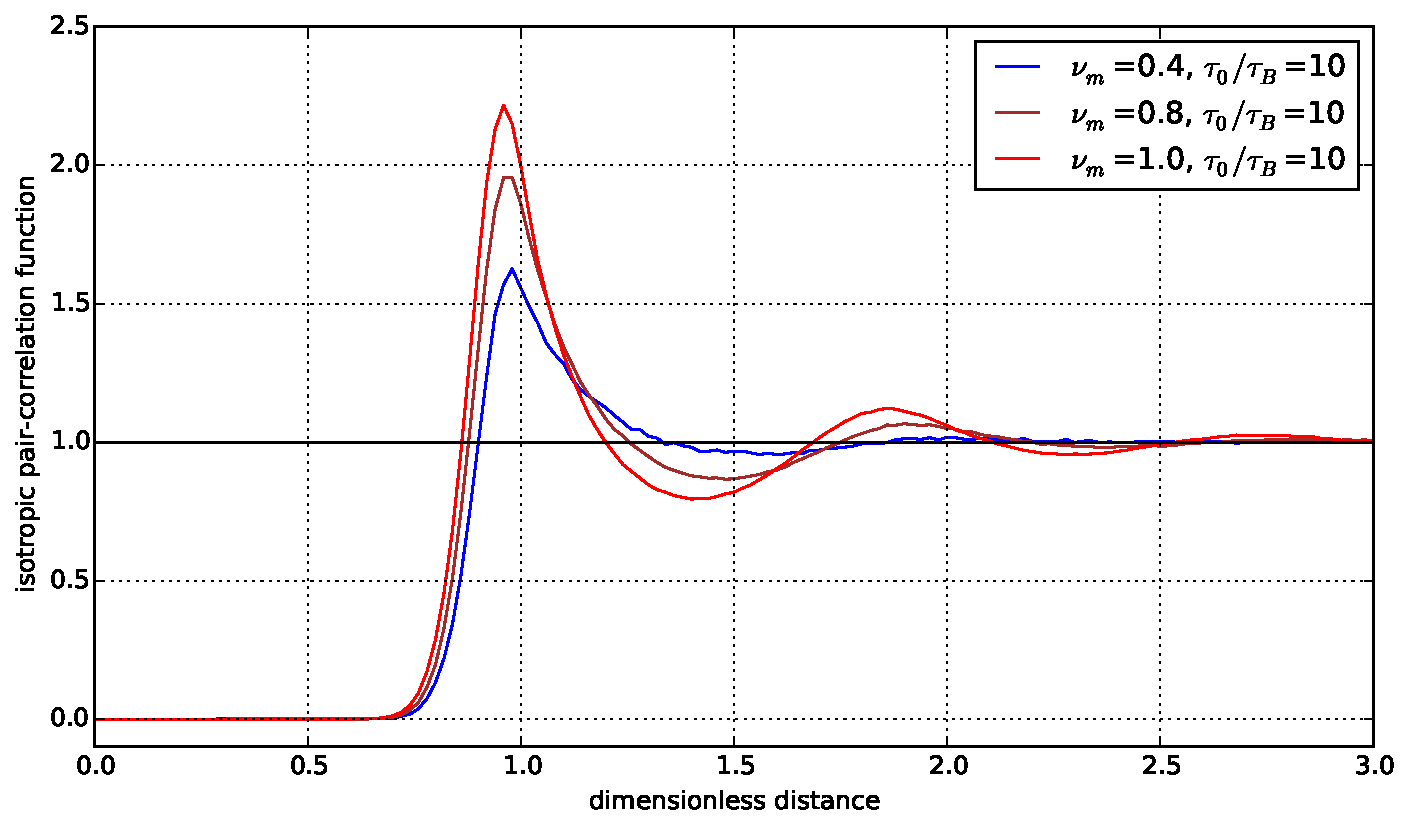
\includegraphics[width=0.8\textwidth]{figures/RDF_compare.pdf}
%%     \caption{Isotropic pair-correlation function account for all the pairs of micelles.}
%%   \end{figure}
%% \end{frame}

%% \begin{frame}
%%   \frametitle{Diffusion Time for Micelles}
%%   \begin{minipage}{0.45\textwidth}
%%     \begin{figure}
%%       \centering
%%       \includegraphics[width=\textwidth]{figures/compare_MSD.pdf}
%%     \end{figure}
%%   \end{minipage}
%%   \begin{minipage}{0.53\textwidth}
%%     \begin{figure}
%%       \centering
%%       \includegraphics[width=\textwidth]{figures/compare_diffusion_coefficient.pdf}
%%       \caption{MSD comparison for pure Brownian, repulsive Brownian, and topological interaction (left), and dimensionless diffusion coefficient with respect to micelle number density, $\nu_m$ (right). }
%%     \end{figure}
%%   \end{minipage}
%% \end{frame}


%% \begin{frame}
%% \frametitle{Stress Autocorrelation: $\tau_0/\tau_B = 1$}
%% \begin{figure}
%%   \centering
%%   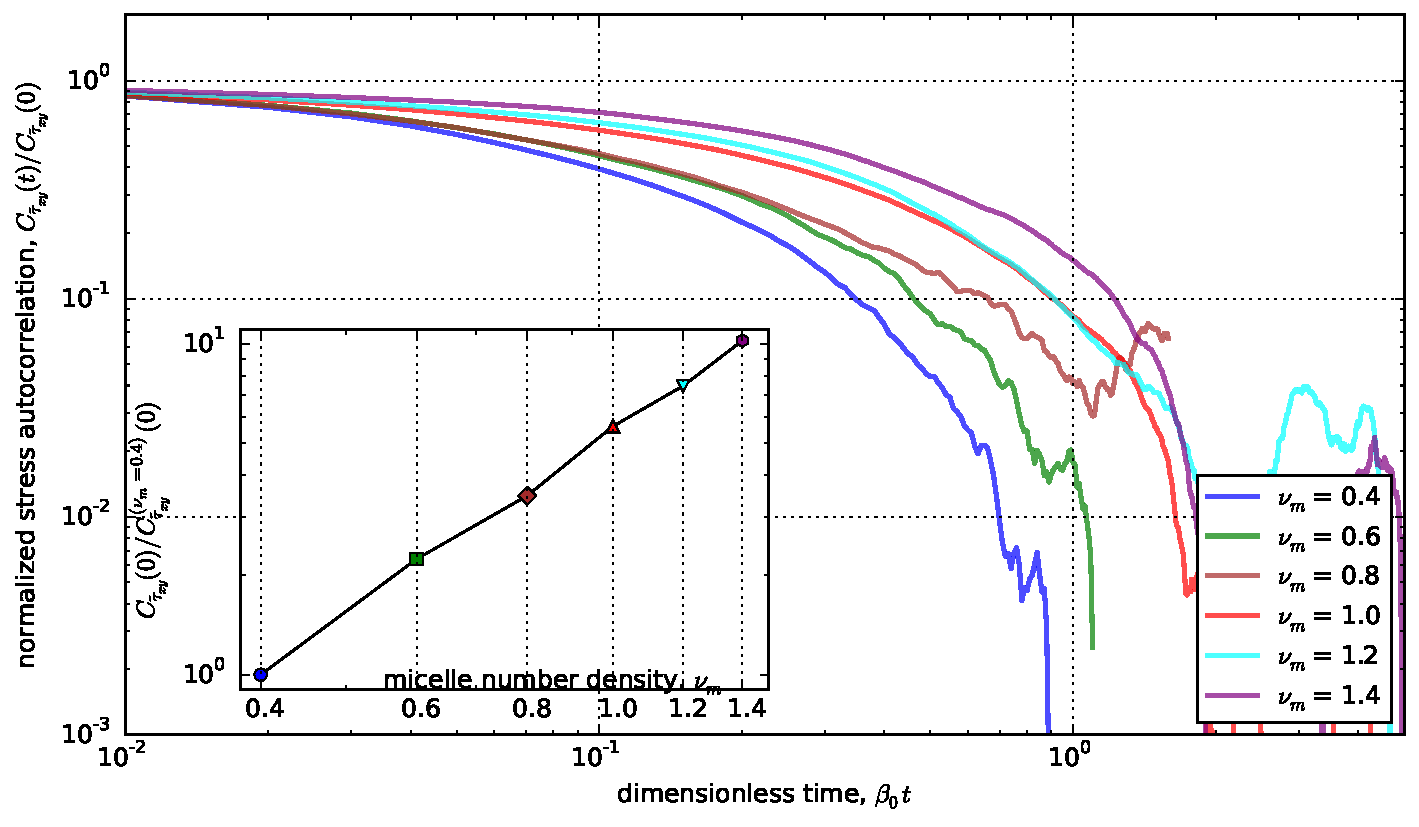
\includegraphics[height=0.7\textheight]{figures/ACF_correction_RT1.pdf}
%%   \caption{Normalized stress autocorrelation for $\tau_0/\tau_B = 1$.}
%% \end{figure}
%% \end{frame}

%% \begin{frame}
%% \frametitle{Stress Autocorrelation: $\tau_0/\tau_B = 10$}
%% \begin{figure}
%%   \centering
%%   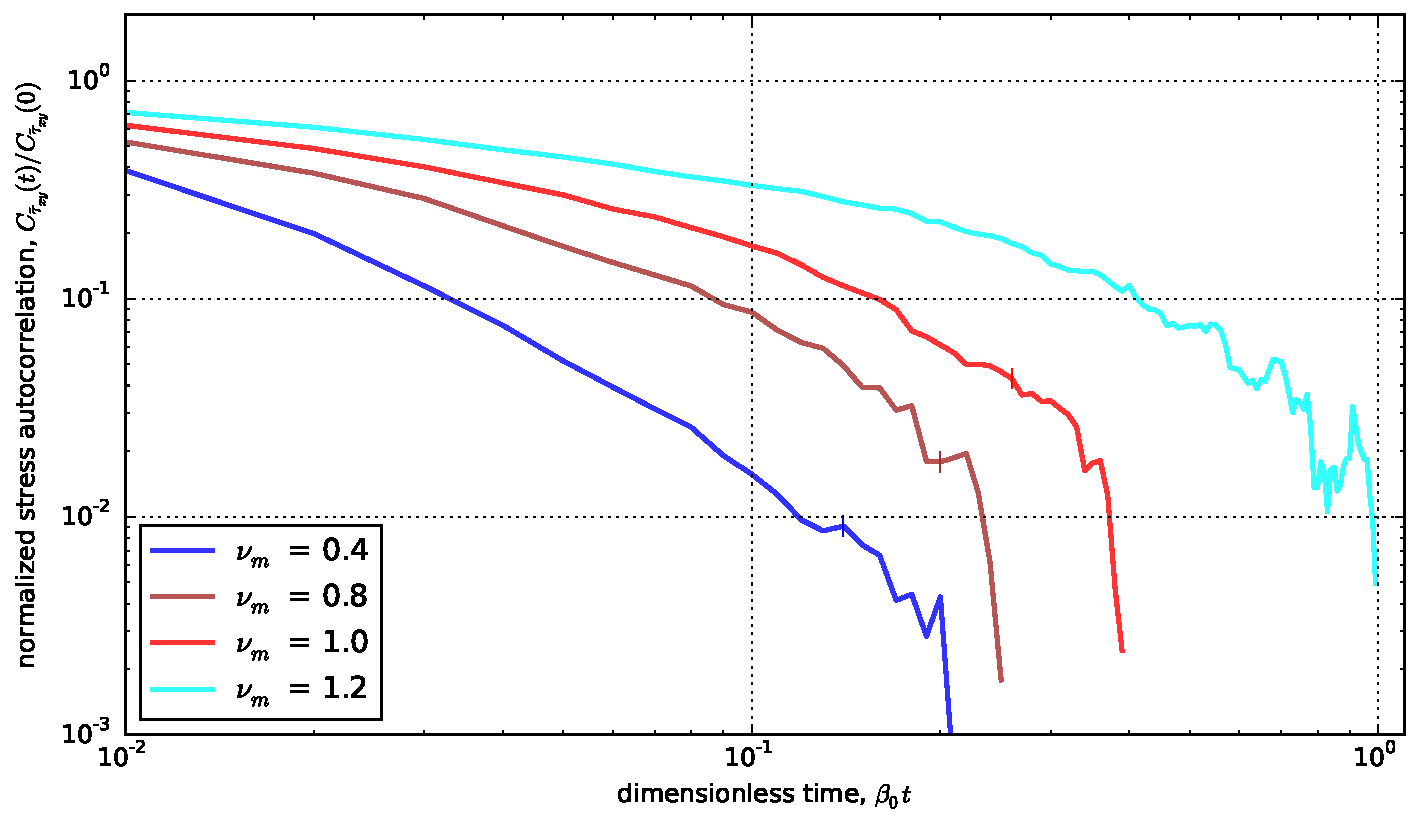
\includegraphics[height=0.7\textheight]{figures/ACF_stress_correction_RT10.pdf}
%%   \caption{Normalized stress autocorrelation for $\tau_0/\tau_B = 10$.}
%% \end{figure}
%% \end{frame}

%% \begin{frame}
%% \frametitle{Stress Autocorrelation: $\nu_m=1$}
%% \begin{figure}
%%   \centering
%%   \includegraphics[height=0.7\textheight]{figures/compare_ACF_NP1000.pdf}
%%   \caption{Normalized stress autocorrelation for $\nu_m=1$.}
%% \end{figure}
%% \end{frame}


%% \section{Conclusions}
%% \begin{frame}
%% \frametitle{Conclusions and Remarks}
%% \begin{itemize}
%% \item Detailed mechanisms of shear thickening for HEUR solution are still controversial
%% \item Anisotropic flow-induced collisions among micelles are regarded as the mechanism for shear thickening and strain hardening for transient viscosity 
%% \item Frictional and topological time scales are well seperated to use decoupled time evolution, which is easily understood by relaxation time spectrum using dynamic moduli in LVE
%% \item Stress autocorrelation shows the scaling law for its intensity with respect to concentration, but the noise make difficult to measure the scaling law for effective relaxation time
%% \end{itemize}
%% \end{frame}

%% % \section{References}
%% \begin{frame}[allowframebreaks]
%%   \frametitle{Bibliography}
%%   \printbibliography[nottype=url]
%% \end{frame}

%% \end{document}

%% % \section{Overview}
%% % \begin{frame}
%% % \frametitle{Models for Transient Networks System \hfill[Crete]}
%% % \begin{block}{Telechelic association system \parencite{Vaccaro:2000}}
%% %   Evolution for attachment and detachment probability are represented by
%% %   \begin{small}\begin{align}
%% %     \frac{\partial }{\partial t}\Psi_{A} &= -\frac{\partial}{\partial \mathbf{R}}\cdot \mathbf{V}_{A} - \beta \Psi_A + \alpha \Psi_D;\\
%% %     \frac{\partial }{\partial t}\Psi_{D} &= -\frac{\partial}{\partial \mathbf{R}}\cdot \mathbf{V}_{D} + \beta \Psi_A - \alpha \Psi_D,
%% %     \end{align}\end{small}
%% %   where $\alpha$ and $\beta$ are kinetic functions.
%% %   % where $\alpha$ and $\beta$ are kinetic functions related to association and dissociation.
%% % \end{block}
%% % \centering\begin{small}\begin{tabular}{|c|c|c|}\hline
%% %       Association($\alpha$) & Dissociation($\beta$) & \multicolumn{1}{c|}{Ref. \parencite{Tripathi:2006}}\\ \hline
%% %       $1/\tau_E$ & $1/\tau_E$ & \small\textcite{Green:1946} \\ \hline
%% %       $c_1\tau_E$ & $\exp(c_2R)/\tau_E$ & \small\textcite{Tanaka:1992_a, Tanaka:1992_b, Tanaka:1992_c} \\ \hline
%% %       $(c_1 R/R_0)/\tau_E$ & $2/\tau_E$ & \small\textcite{VandenBrule:1995}\\ \hline
%% %       $ (c_1 + c_2R/R_0)/\tau_E$ & $f/\tau_E$ & \small\textcite{Vaccaro:2000} \\ \hline
%% %     \end{tabular}\end{small}
%% % \end{frame}

%% % %% \begin{frame}
%% % %%   \frametitle{Simulation for Transient Networks System\hfill[Geleen]}
%% % %%   \begin{block}{Coarse-Grained Models}
%% % %%     \begin{itemize}
%% % %%     \item \textcite{Koga:2005kz}: introduce individual sticky bead
%% % %%     \item \textcite{Hoy:2009}: stochastic decision for association/dissociation
%% % %%     \item \textcite{Li:2010bm}: control long-range interaction for donor and acceptor beads
%% % %% % Using attractive bead \parencite{Koga:2005kz, Li:2010bm}
%% % %% %     \item Using stochastic decision for associative bond \parencite{Hoy:2009}
%% % %%     \end{itemize}
%% % %%   \end{block}
%% % %%   \begin{block}{Atomistic Molecular Dynamics}
%% % %%     \begin{itemize}
%% % %%     \item Association/dissociation mechanics is naturally builted-in based for given force field
%% % %%     \item Time and length scales are restricted 
%% % %%     \end{itemize}
%% % %%   \end{block}
%% % %% \end{frame}

%% % \begin{frame}
%% %   \frametitle{Atomistic Molecular Dynamics for Oligomer \hfill[Geleen]}
%% %   \begin{block}{Without association: Flow induced friction reduction}
%% %     \begin{itemize}
%% %     \item Non-equilibrium MD (NEMD) simulation: steady shear flow with high flow rate ($\dot{\gamma} \geq \tau_R^{-1}$)
%% %     \item Measure mobility($\mathbf{M}$), friction($\boldsymbol{\zeta}$), and diffusivity($\mathbf{D}$)
%% %     \item Chemical dependency for friction reduction: Oligomer type PS, PMMA, PnBA
%% %     \end{itemize}
%% %   \end{block}
%% %   \begin{block}{With association: Flow effects to the kinetic functions}
%% %     \begin{itemize}
%% %     \item Introduce sticky group for oligomer using TraPPE-UA force field
%% %     \item Observe time scales for associative system and tuning using temperature controls
%% %     \item Development the method to measure the kinetics
%% %     \end{itemize}
%% %   \end{block}
%% % \end{frame}

%% % \section{Methodology}

%% % \begin{frame}
%% %   \frametitle{Generating Initial Box for Oligomer}
%% %   \begin{minipage}{0.6\textwidth}
%% %   \begin{enumerate}
%% %   \item Set the system and building molecules: SMILES string $\Rightarrow$ 3d structure
%% %   \item Developing force fields based on TraPPE-UA force field
%% %     \begin{itemize}
%% %     \item Tree data structure for connected atoms
%% %     \item Generating all connections for the force field using pre-order tree traversal method
%% %     \item Generating all types for non-bonding potential
%% %     \end{itemize}
%% %   \item Equilibration
%% %   \item Optimization computation efficiency
%% %   \end{enumerate}
%% %   \end{minipage}
%% %   \begin{minipage}{0.38\textwidth}
%% %     \begin{figure}
%% %       \centering
%% %       \includegraphics[width=\textwidth]{figures/preorder_tree.pdf}
%% %       \caption{\small{Schematic diagram for pre-order travel for tree structure.}}
%% %     \end{figure}
%% %   \end{minipage}
%% % \end{frame}

%% % \begin{frame}
%% %   \frametitle{TraPPE-UA force fields for PMMA and PnBA}
%% %   \begin{block}{Bonded interactions}
%% %     \begin{enumerate}
%% %     \item Rigid bonding potential: $u_{12}(r) = l_0$
%% %     \item Simple harmonic angle potential: $u_{13}(\theta) = \frac{k_\theta}{2}\left(\theta-\theta_0\right)^2$
%% %     \item Dihedral potential: $V_n(\phi)=k_{\phi}(1+\cos(n\phi-\phi_s))$
%% %     \end{enumerate}
%% %   \end{block}
%% %   \begin{block}{Non-bonded interaction}
%% %     \begin{enumerate}
%% %     \item Lennard-Jones 6-12 potentials with long-range correction
%% %     \item Coulomb potential for electrostatic using Particle-Mesh Ewald Sum (PME)
%% %     \end{enumerate}
%% %   \end{block}
%% %   All the detail parameters are extracted by \textcite{Maerzke:2009, Kamath:2006, Stubbs:2004, Sokkalingam:2009, Ferrando:2012}.
%% % \end{frame}


%% % \begin{frame}
%% %   \frametitle{Diffusivity and Mean Square Displacement}
%% %   \vspace{-0.2in}
%% %   \begin{figure}
%% %     \hspace{-0.5in}
%% %     \begin{minipage}[b]{0.75\textwidth}
%% %       \centering
%% %       \includegraphics[width=\textwidth]{figures/msd_compare_AHT_SHT_REF.pdf}
%% %     \end{minipage}
%% %     \hspace{-0.3in}
%% %     \begin{minipage}[b]{0.3\textwidth}
%% %       \caption{\small{Mean-square displacement for PMMA decamer and comparison with \textcite{Chen:2008ec}. The symbol is for reference data, solid line represent NVT simulation with typical PMMA density, and dashed lines are NPT simulationa.}}
%% %     \end{minipage}
%% %   \end{figure}
%% % \end{frame}


%% % \begin{frame}
%% %   \frametitle{Time Scales and Computation Limitations}
%% %   \vspace{-0.1in}
%% %   \begin{block}{Correlation function for end-to-end vector}
%% %     Let $\mathbf{P}(t)$ is end-to-end vector for a molecule, the correlation is given by
%% %     \begin{equation}
%% %       Corr[\mathbf{P}, \mathbf{P}](t) = \langle \mathbf{P}(\xi)\cdot\mathbf{P}(\xi + t)\rangle_{\xi} \propto \exp\left(-\frac{t}{\tau_R}\right)\textrm{ for }t \geq \tau_R,
%% %     \end{equation}
%% %     where $\tau_R$ is the longest characteristic time for the end-to-end vector.
%% %   \end{block}
%% %   \vspace{-0.1in}
%% %   \begin{figure}
%% %     \begin{minipage}[b]{0.50\textwidth}
%% %       \centering
%% %       \includegraphics[width=0.83\textwidth]{figures/acf_500_600.pdf}
%% %     \end{minipage}
%% %     \begin{minipage}[b]{0.40\textwidth}
%% %       \caption{\small{Results of autocorrelation function for PMMA decamer at 500K and 600K. The plot represents almost single exponential decay which make simple to calculation characteristic time.}}
%% %     \end{minipage}
%% %   \end{figure}
%% % \end{frame}


%% % \begin{frame}
%% %   \frametitle{Constant Pulling for Mobility and Friction Tensors}
%% %   \begin{block}{Mobility Tensor}
%% %     Because of isotropic nature of the system, the long-time average for velocity and force exerted on the pulled molecule can be presented by 
%% %     \begin{small}\begin{equation}
%% %       \langle \mathbf{v}\rangle_{t, p} = \mathbf{M}\cdot\langle\mathbf{f}\rangle,\label{eq:mobility}
%% %     \end{equation}\end{small}
%% %     where $\mathbf{M}$ is mobility tensor, $\mathbf{f}$ is pulling constant, and $t$ and $p$ denote the average taking over the time and pulled molecules.
%% %   \end{block}
%% %   In equilibrium, when pulling force is appropriately choose, the diffusion coefficient, $D_{eq}$, and mobility, $M_{eq}$, can be connected by Einstein-Stokes relation:
%% %   \small{\begin{equation}
%% %     D_{eq} = k_BT M_{eq},\label{eq:einstein_stokes}.
%% %   \end{equation}}

%% % \end{frame}

%% % \begin{frame}
%% %   \frametitle{Constant Pulling for Mobility and Friction Tensors (cont.)}
%% %   \begin{figure}
%% %     \centering
%% %     \includegraphics[width=0.49\textwidth]{figures/X_components_for_pulled_molecule.pdf}
%% %     \includegraphics[width=0.49\textwidth]{figures/diffusivity_compare.pdf}
%% %     \caption{\small{(left) X trajectory for pulled molecules with different pulling force. (right) Calculated diffusion coefficient in equilibrium from average mean-square-displacement for unpulled molecule (blue symbol) and converted diffusion coefficient using Einstein-Stokes relation (red symbol).}}
%% %   \end{figure}
%% % \end{frame}




%% % \begin{frame}
%% %   \frametitle{Boundary Driven Algorithm for Steady Shear Flow}
%% %   \vspace{-0.1in}
%% %   \begin{figure}
%% %     \begin{minipage}[b]{0.5\textwidth}
%% %       \centering
%% %       \includegraphics[width=0.8\textwidth]{figures/boundary_driven_shear.png}
%% %     \end{minipage}
%% %     \begin{minipage}[b]{0.45\textwidth}
%% %       \caption{\small{Schematic diagram to depict boundary driven shear flow so-called Lee-Edwards sliding bricks. This is valid for time independent flow.}}
%% %     \end{minipage}
%% %   \end{figure}
%% %   \vspace{-0.1in}
%% %   The Lagrangian coordinate for the trajectory is results of following correction:
%% %     \begin{equation}
%% %       X_{CM}^{\ast(k)}(t) = X_{CM}^{(t)}(t) - \dot{\gamma}\int_0^t Y_{CM}^{(k)}(t')dt',
%% %     \end{equation}
%% %     where $X_{CM}$, $Y_{CM}$, and $Z_{CM}$ are given xyz components for trajectory.
    
%% % \end{frame}

%% % \section{Conjecture}
%% % \begin{frame}
%% %   \frametitle{Interpretation of Time Scales}
%% %   \begin{minipage}[b]{0.5\textwidth}
%% %     \begin{block}{Tuning temperature for PMMA}
%% %       \begin{itemize}
%% %       \item Tg for PMMA around 380K (atatic)
%% %       \item Density for PMMA is around 1.066 (g/cm$^3$)
%% %       \item 100 decamer (PMMA):
%% %         \begin{itemize}
%% %         \item 1-2 ns for 1 hour
%% %         \item For $\tau_R\approx 10$(ns), 200-300ns\\ $\Rightarrow$ 10-20 days
%% %         \end{itemize}
%% %       \item From 500K to 600K:
%% %         \begin{itemize}
%% %         \item density: 1.03 $\rightarrow$ 0.96 (g/cm$^3$)
%% %         \item $\tau_R$: 8.8 $\rightarrow$ 1.2 (ns)
%% %         \end{itemize}
%% %       \end{itemize}
%% %     \end{block}
%% %   \end{minipage}
%% %   \hspace{0.1in}
%% %   \begin{minipage}[b]{0.4\textwidth}
%% %     \begin{figure}
%% %       \includegraphics[width=\textwidth]{figures/shift_factor_anal_PMMA.pdf}
%% %       \caption{\small{Interpretation of time scales and density profiles with respect to temperature. The expected scheme is followed typical PMMA data.}}
%% %     \end{figure}
%% %   \end{minipage}
%% % \end{frame}

%% % \begin{frame}
%% %   \frametitle{Interpretation of Time Scales for PnBA with Association}
%% %   \vspace{-0.1in}
%% %   \begin{block}{PnBA + Association}
%% %     \begin{itemize}
%% %     \item At 373K, time scale is around 10ns (Tg for PnBA is around 200K)
%% %     \item Longer relaxation time for associative system
%% %     \item Different temperature dependence for association and oligomer dynamics
%% %     \end{itemize}
%% %   \end{block}
%% %   \begin{figure}
%% %   \begin{minipage}{0.7\textwidth}
%% %     \includegraphics[width=\textwidth]{figures/pba_association.png}
%% %   \end{minipage}
%% %   \begin{minipage}{0.25\textwidth}
%% %     \caption{PnBA with hydrogen bonding side group with different bonding strength \parencite{Lewis:2014fs}.}
%% %   \end{minipage}
%% %   \end{figure}
%% % \end{frame}

%% % \section{Conclusions}
%% % \begin{frame}
%% %   \frametitle{Summary and Future Works}
%% %   \begin{enumerate}
%% %   \item The research object is effects of flow to the kinetic functions
%% %   \item For the simplicity of implementation for differemt material systems, atomistic MD simulation is selcted 
%% %   \item For steady shear flow, the sliding bricks concept make easy to implement for PBC
%% %   \item For computational limitation, the longest relaxation time for end-to-end vector should be around 10 ns
%% %   \item Effects of temperature to the oligomer dynamics and association/dissociation kinetics has different role that make difficulty to tuning time scales of the system
%% %   \item When objective system has outside of processing time scales, coarse-grained simulation is under the consideration to perform
%% %   \end{enumerate}
%% % \end{frame}


